% answers.tex —— 2016 年·浙江卷·理科 · 参考答案与详细解析片段
% 由 tools/generate_projects.py 依来源总账自 2016/2016_数学真题_浙江理_试题.md + 2016/2016_数学真题_浙江理_解析正文.md + 2016/2016_数学真题_浙江理_答案要点.md 生成，勿手改（改源 MD 后重跑）


\begin{gktip}
固定原卷不附官方答案。以下为独立推导并经异人盲核对照的解析（非官方答案，等级 D）。第 6 题点列图的阴影三角形、第 11 题三视图的几何构型与第 17 题三棱台的顶点位置均已按源图矢量数据复核；第 11 题的体积与表面积在两种投影约定（互为镜像）下不变。第 16 题（2）有两解，均代回题设验证成立。
\end{gktip}

\begin{answer}
\gksolhead{1}{}

\textbf{题目}：

已知集合 \(P=\{x\in\mathbf{R}\mid 1\leqslant x\leqslant 3\}\)，\(Q=\{x\in\mathbf{R}\mid x^{2}\geqslant 4\}\)，则 \(P\cup(\complement_{\mathbf{R}}Q)=\)（　）

（A）\([2,3]\)　（B）\((-2,3]\)　（C）\([1,2)\)　（D）\((-\infty,-2]\cup[1,+\infty)\)

\Needspace{4\baselineskip}
\textbf{解析}

由 \(x^{2}\geqslant 4\) 得 \(Q=(-\infty,-2]\cup[2,+\infty)\)，故 \(\complement_{\mathbf{R}}Q=(-2,2)\)；又 \(P=[1,3]\)，故 \(P\cup(\complement_{\mathbf{R}}Q)=(-2,2)\cup[1,3]=(-2,3]\)。

\gkanswer{答案：B，\((-2,3]\)}

\end{answer}
\begin{answer}
\gksolhead{2}{}

\textbf{题目}：

已知互相垂直的平面 \(\alpha\)，\(\beta\) 交于直线 \(l\)，若直线 \(m\)，\(n\) 满足 \(m\parallel\alpha\)，\(n\perp\beta\)，则（　）

（A）\(m\parallel l\)　（B）\(m\parallel n\)　（C）\(n\perp l\)　（D）\(m\perp n\)

\Needspace{4\baselineskip}
\textbf{解析}

由 \(\alpha\perp\beta\)，\(l=\alpha\cap\beta\)，得 \(l\subset\beta\)；由 \(n\perp\beta\) 得 \(n\) 垂直于平面 \(\beta\) 内的每一条直线，特别地 \(n\perp l\)。

（其余选项排除：\(m\parallel\alpha\) 与 \(l\) 无必然关系；\(\alpha\perp\beta\) 时 \(n\parallel\alpha\)，但两条直线同平行于一平面不能推出 \(m\parallel n\)，故 (A)(B)(D) 均不一定成立。）

\gkanswer{答案：C，\(n\perp l\)}

\end{answer}
\begin{answer}
\gksolhead{3}{}

\textbf{题目}：

在平面上，过点 \(P\) 作直线 \(l\) 的垂线所得的垂足称为点 \(P\) 在直线 \(l\) 上的投影。由区域 \(\begin{cases} x-2\leqslant 0, \\ x+y\geqslant 0, \\ x-3y+4\geqslant 0 \end{cases}\) 中的点在直线 \(x+y-2=0\) 上的投影构成的线段记为 \(AB\)，则 \(|AB|=\)（　）

（A）\(2\sqrt{2}\)　（B）4　（C）\(3\sqrt{2}\)　（D）6

\Needspace{4\baselineskip}
\textbf{解析}

可行域由 \(x\leqslant 2\)、\(y\geqslant -x\)、\(y\leqslant\dfrac{x+4}{3}\) 围成三角形，三顶点为 \((2,-2)\)，\((2,2)\)，\((-1,1)\)。

\Needspace{5\baselineskip}
投影沿直线 \(x+y-2=0\) 的法向 \((1,1)\) 进行，此方向上 \(x-y\) 不变，沿直线方向取坐标 \(u=\dfrac{x-y}{\sqrt{2}}\)。三顶点处 \(x-y\) 的值分别为 \(4,0,-2\)，故

\nopagebreak[4]
\[
|AB|=\dfrac{\max(x-y)-\min(x-y)}{\sqrt{2}}=\dfrac{4-(-2)}{\sqrt{2}}=3\sqrt{2}.
\]

\gkanswer{答案：C，\(3\sqrt{2}\)}

\end{answer}
\begin{answer}
\gksolhead{4}{}

\textbf{题目}：

命题“\(\forall x\in\mathbf{R}\)，\(\exists n\in\mathbf{N}^{*}\)，使得 \(n\geqslant x^{2}\)”的否定形式是（　）

（A）\(\forall x\in\mathbf{R}\)，\(\exists n\in\mathbf{N}^{*}\)，使得 \(n<x^{2}\)　（B）\(\forall x\in\mathbf{R}\)，\(\forall n\in\mathbf{N}^{*}\)，使得 \(n<x^{2}\)　（C）\(\exists x\in\mathbf{R}\)，\(\exists n\in\mathbf{N}^{*}\)，使得 \(n<x^{2}\)　（D）\(\exists x\in\mathbf{R}\)，\(\forall n\in\mathbf{N}^{*}\)，使得 \(n<x^{2}\)

\Needspace{4\baselineskip}
\textbf{解析}

全称命题的否定：量词 \(\forall\) 与 \(\exists\) 互换，结论取反，得 \(\exists x\in\mathbf{R}\)，\(\forall n\in\mathbf{N}^{*}\)，使得 \(n<x^{2}\)。

\gkanswer{答案：D，\(\exists x\in\mathbf{R}\)，\(\forall n\in\mathbf{N}^{\ast}\)，使得 \(n<x^{2}\)}

\end{answer}
\begin{answer}
\gksolhead{5}{}

\textbf{题目}：

设函数 \(f(x)=\sin^{2}x+b\sin x+c\)，则 \(f(x)\) 的最小正周期（　）

（A）与 \(b\) 有关，且与 \(c\) 有关　（B）与 \(b\) 有关，但与 \(c\) 无关　（C）与 \(b\) 无关，且与 \(c\) 无关　（D）与 \(b\) 无关，但与 \(c\) 有关

\Needspace{4\baselineskip}
\textbf{解析}

\(f(x)=\sin^{2}x+b\sin x+c=\dfrac{1-\cos 2x}{2}+b\sin x+c\)。

当 \(b=0\) 时 \(f(x)=\sin^{2}x+c\)，最小正周期为 \(\pi\)；当 \(b\neq 0\) 时 \(f(x+\pi)=\sin^{2}x-b\sin x+c\neq f(x)\)，故 \(\pi\) 不是周期，最小正周期为 \(2\pi\)。即最小正周期与 \(b\) 有关、与 \(c\) 无关。

\gkanswer{答案：B，与 \(b\) 有关，但与 \(c\) 无关}

\end{answer}
\begin{answer}
\gksolhead{6}{}

\textbf{题目}：

如图，点列 \(\{A_{n}\}\)，\(\{B_{n}\}\) 分别在某锐角的两边上，且 \(|A_{n}A_{n+1}|=|A_{n+1}A_{n+2}|\)，\(A_{n}\neq A_{n+2}\)，\(n\in\mathbf{N}^{*}\)，\(|B_{n}B_{n+1}|=|B_{n+1}B_{n+2}|\)，\(B_{n}\neq B_{n+2}\)，\(n\in\mathbf{N}^{*}\)（\(P\neq Q\) 表示点 \(P\) 与 \(Q\) 不重合）。若 \(d_{n}=|A_{n}B_{n}|\)，\(S_{n}\) 为 \(\triangle A_{n}B_{n}B_{n+1}\) 的面积，则（　）
\nopagebreak[4]
\begin{center}% 第 6 题点列图：按固定源 PDF 矢量路径换算（1 pt → 0.03515 cm）。
% 原点取下边射线的左端（源页 (155.6289, 652.3750) pt），y 向上。
% 两条截断射线（角顶点在图外，源图有意不画）；三个浅灰填充三角形 S1/S2/Sn；
% 点列 A1..A(n+1) 在上射线、B1..B(n+1) 在下水平线（等距 20.22 pt）；16 组文字标签。
% 注：两射线已画端点纵向相距 23.05 pt、横向错开仅 0.40 pt（被同一竖直截断线切齐），
% 判为有意截断（交点外推约 (114.5, 652.4)），照源复刻不补顶点。
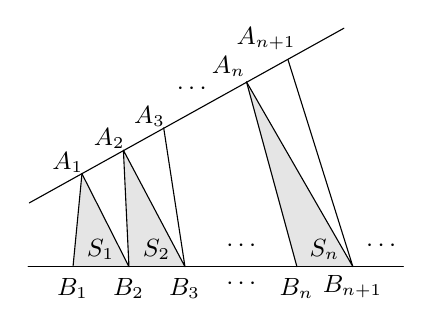
\begin{tikzpicture}[line cap=round,line join=round,font=\small,x=0.03515cm,y=0.03515cm]
% ===== 浅灰填充三角形（fill-opacity 0.1）=====
\fill[black,fill opacity=0.1] (19.41,33.57)--(16.18,0)--(36.39,0)--cycle;
\fill[black,fill opacity=0.1] (34.38,42.06)--(56.62,0)--(36.39,0)--cycle;
\fill[black,fill opacity=0.1] (78.86,66.73)--(97.06,0)--(117.28,0)--cycle;
% ===== 线画 =====
\draw (135.48,0)--(0,0);                 % 下边（水平射线，B 点列所在）
\draw (114.04,86.14)--(0.40,23.05);      % 上边（斜射线，A 点列所在）
\draw (19.41,33.57)--(16.18,0);          % A1B1
\draw (19.41,33.57)--(36.39,0)--(34.38,42.06)--(56.62,0)--(48.93,50.15);  % A1→B2→A2→B3→A3
\draw (78.86,66.73)--(97.06,0);          % AnBn
\draw (78.86,66.73)--(117.28,0)--(93.82,74.82);  % An→Bn+1→An+1
% ===== 文字标签（照源字形框中心，显式坐标）=====
\node[anchor=center,inner sep=0] at (14.30,37.75) {\(A_{1}\)};
\node[anchor=center,inner sep=0] at (29.27,46.25) {\(A_{2}\)};
\node[anchor=center,inner sep=0] at (43.83,54.34) {\(A_{3}\)};
\node[anchor=center,inner sep=0] at (59.05,64.27) {\(\cdots\)};
\node[anchor=center,inner sep=0] at (72.36,72.33) {\(A_{n}\)};
\node[anchor=center,inner sep=0] at (85.92,82.25) {\(A_{n+1}\)};
\node[anchor=center,inner sep=0] at (26.11,6.21) {\(S_{1}\)};
\node[anchor=center,inner sep=0] at (46.34,6.21) {\(S_{2}\)};
\node[anchor=center,inner sep=0] at (76.93,7.65) {\(\cdots\)};
\node[anchor=center,inner sep=0] at (107.02,6.21) {\(S_{n}\)};
\node[anchor=center,inner sep=0] at (127.50,7.65) {\(\cdots\)};
\node[anchor=center,inner sep=0] at (15.99,-7.74) {\(B_{1}\)};
\node[anchor=center,inner sep=0] at (36.22,-7.74) {\(B_{2}\)};
\node[anchor=center,inner sep=0] at (56.45,-7.74) {\(B_{3}\)};
\node[anchor=center,inner sep=0] at (76.93,-6.30) {\(\cdots\)};
\node[anchor=center,inner sep=0] at (96.91,-7.74) {\(B_{n}\)};
\node[anchor=center,inner sep=0] at (117.13,-7.32) {\(B_{n+1}\)};
\end{tikzpicture}
\end{center}
\nopagebreak[4]
（A）\(\{S_{n}\}\) 是等差数列　（B）\(\{S_{n}^{2}\}\) 是等差数列　（C）\(\{d_{n}\}\) 是等差数列　（D）\(\{d_{n}^{2}\}\) 是等差数列

\Needspace{4\baselineskip}
\textbf{解析}

\Needspace{5\baselineskip}
设两射线夹角为 \(\theta\)，\(u_{n}=|OA_{n}|\)，\(v_{n}=|OB_{n}|\)。由等距条件，\(\{u_{n}\}\)、\(\{v_{n}\}\) 均为等差数列，设 \(v_{n+1}-v_{n}=q>0\)。因 \(B_{n}\) 在线段 \(OB_{n+1}\) 上，

\nopagebreak[4]
\[
S_{n}=[\triangle OA_{n}B_{n+1}]-[\triangle OA_{n}B_{n}]=\dfrac{1}{2}u_{n}v_{n+1}\sin\theta-\dfrac{1}{2}u_{n}v_{n}\sin\theta=\dfrac{1}{2}q\sin\theta\cdot u_{n}.
\]

\(u_{n}\) 是 \(n\) 的等差数列，故 \(S_{n}\) 是等差数列。

（\(d_{n}^{2}=u_{n}^{2}+v_{n}^{2}-2u_{n}v_{n}\cos\theta\) 是 \(n\) 的二次式，其二次项系数 \((p-q)^{2}+2pq(1-\cos\theta)>0\)，故 \(\{d_{n}\}\)、\(\{d_{n}^{2}\}\)、\(\{S_{n}^{2}\}\) 均非等差数列。）

\gkanswer{答案：A，\(\{S_{n}\}\) 是等差数列}

\end{answer}
\begin{answer}
\gksolhead{7}{}

\textbf{题目}：

已知椭圆 \(C_{1}:\dfrac{x^{2}}{m^{2}}+y^{2}=1\)（\(m>1\)）与双曲线 \(C_{2}:\dfrac{x^{2}}{n^{2}}-y^{2}=1\)（\(n>0\)）的焦点重合，\(e_{1}\)，\(e_{2}\) 分别为 \(C_{1}\)，\(C_{2}\) 的离心率，则（　）

（A）\(m>n\) 且 \(e_{1}e_{2}>1\)　（B）\(m>n\) 且 \(e_{1}e_{2}<1\)　（C）\(m<n\) 且 \(e_{1}e_{2}>1\)　（D）\(m<n\) 且 \(e_{1}e_{2}<1\)

\Needspace{4\baselineskip}
\textbf{解析}

椭圆 \(C_{1}\) 的半焦距满足 \(c_{1}^{2}=m^{2}-1\)，双曲线 \(C_{2}\) 满足 \(c_{2}^{2}=n^{2}+1\)。由焦点重合得 \(m^{2}-1=n^{2}+1\)，即 \(m^{2}-n^{2}=2\)，故 \(m>n\)。

\Needspace{5\baselineskip}
记 \(k=m^{2}-1=n^{2}+1\)，则 \(e_{1}e_{2}=\dfrac{\sqrt{m^{2}-1}\cdot\sqrt{n^{2}+1}}{mn}=\dfrac{k}{mn}\)。由 \(m^{2}-n^{2}=2\) 得 \(m-n=\dfrac{2}{m+n}\)，于是

\nopagebreak[4]
\[
e_{1}e_{2}>1\iff m^{2}-1>mn\iff m(m-n)>1\iff\dfrac{2m}{m+n}>1\iff m>n,
\]

最后一步恒成立，故 \(e_{1}e_{2}>1\)。

\gkanswer{答案：A，\(m>n\) 且 \(e_{1}e_{2}>1\)}

\end{answer}
\begin{answer}
\gksolhead{8}{}

\textbf{题目}：

已知实数 \(a\)，\(b\)，\(c\)。（　）

（A）若 \(|a^{2}+b+c|+|a+b^{2}+c|\leqslant 1\)，则 \(a^{2}+b^{2}+c^{2}<100\)　（B）若 \(|a^{2}+b+c|+|a^{2}+b-c|\leqslant 1\)，则 \(a^{2}+b^{2}+c^{2}<100\)

（C）若 \(|a+b+c^{2}|+|a+b-c^{2}|\leqslant 1\)，则 \(a^{2}+b^{2}+c^{2}<100\)　（D）若 \(|a^{2}+b+c|+|a+b^{2}-c|\leqslant 1\)，则 \(a^{2}+b^{2}+c^{2}<100\)

\Needspace{4\baselineskip}
\textbf{解析}

\Needspace{5\baselineskip}
取 (D)：设 \(X=a^{2}+b+c\)，\(Y=a+b^{2}-c\)，由 \(|X|+|Y|\leqslant 1\) 得

\nopagebreak[4]
\[
|a^{2}+a+b^{2}+b|=|X+Y|\leqslant 1\Longrightarrow\left(a+\dfrac{1}{2}\right)^{2}+\left(b+\dfrac{1}{2}\right)^{2}\leqslant\dfrac{3}{2}.
\]

故 \(|a|\leqslant\dfrac{1}{2}+\sqrt{\dfrac{3}{2}}\)，\(|b|\) 同理，从而 \(a^{2}+b^{2}\leqslant 2\left(\dfrac{1}{2}+\sqrt{\dfrac{3}{2}}\right)^{2}\)；又 \(|c|\leqslant|Y|+|a|+b^{2}\)，得 \(c^{2}\) 有上界。合计 \(a^{2}+b^{2}+c^{2}<100\)，(D) 恒成立。

（(A)(B)(C) 均可用反例排除，如 (A) 取 \(a=b=10\)，\(c=-110\)：前提成立而 \(a^{2}+b^{2}+c^{2}>100\)。）

\gkanswer{答案：D}

\end{answer}
\begin{answer}
\gksolhead{9}{}

\textbf{题目}：

若抛物线 \(y^{2}=4x\) 上的点 \(M\) 到焦点的距离为 10，则 \(M\) 到 \(y\) 轴的距离是 \(\underline{\qquad}\)。

\Needspace{4\baselineskip}
\textbf{解析}

\(y^{2}=4x\) 的焦点为 \((1,0)\)，准线为 \(x=-1\)。抛物线上的点到焦点的距离等于到准线的距离，故 \(x_{M}+1=10\)，即 \(x_{M}=9\)。点 \(M\) 到 \(y\) 轴的距离为 \(9\)。

\gkanswer{答案：\(9\)}

\end{answer}
\begin{answer}
\gksolhead{10}{}

\textbf{题目}：

已知 \(2\cos^{2}x+\sin 2x=A\sin(\omega x+\varphi)+b\)（\(A>0\)），则 \(A=\) \(\underline{\qquad}\)，\(b=\) \(\underline{\qquad}\)。

\Needspace{4\baselineskip}
\textbf{解析}

\Needspace{5\baselineskip}
由 \(2\cos^{2}x=1+\cos 2x\) 得

\nopagebreak[4]
\[
2\cos^{2}x+\sin 2x=1+(\cos 2x+\sin 2x)=1+\sqrt{2}\sin\left(2x+\dfrac{\pi}{4}\right).
\]

与 \(A\sin(\omega x+\varphi)+b\)（\(A>0\)）对照得 \(A=\sqrt{2}\)，\(b=1\)。

\gkanswer{答案：\(A=\sqrt{2}\)，\(b=1\)}

\end{answer}
\begin{answer}
\gksolhead{11}{}

\textbf{题目}：

某几何体的三视图如图所示（单位：cm），则该几何体的表面积是 \(\underline{\qquad}\) cm²，体积是 \(\underline{\qquad}\) cm³。
\nopagebreak[4]
\begin{center}% 第 11 题三视图：按固定源 PDF 矢量路径换算（1 pt → 0.03515 cm）。
% 原点取正视图左下角（源页 (524.5664, 375.2969) pt），y 向上。网格 28.1953 pt = 2 cm。
% 正视图：2×2 格、左上格缺（中竖贯通、中横仅左半）；侧视图：2×2 格、右下格缺（中横贯通、
% 中竖下半为虚线——源内线型如此，按源照录）；俯视图：左列满深、右列只余上半。
% 尺寸标注：横向 4 条 + 竖向 2 条尺寸线（均两段让位给数字），6 条竖直刻度线、3 条水平刻度线，
% 12 个实心箭头（横向一律朝外）；「2」「正视图」「侧视图」「俯视图」共 9 个标签。
\begin{tikzpicture}[line cap=round,line join=round,font=\small,x=0.03515cm,y=0.03515cm]
% ===== 正视图（左格）=====
\draw (0,0)--(56.39,0)--(56.39,56.39)--(28.20,56.39)--(28.20,28.20)--(0,28.20)--cycle;
\draw (28.20,0)--(28.20,28.20);                 % 中竖下半（实线）
% ===== 侧视图（右格，右移 84.58）=====
\draw (84.58,0)--(140.97,0)--(140.97,28.20)--(112.78,28.20)--(112.78,56.39)--(84.58,56.39)--cycle;
\draw (84.58,28.20)--(112.78,28.20);            % 中横左半（实线）
\draw[dash pattern=on 2.99pt off 2.99pt] (112.78,0)--(112.78,28.20);  % 中竖下半（虚线，照源）
% ===== 俯视图 =====
\draw (0,-28.20)--(28.20,-28.20)--(28.20,-84.58)--(0,-84.58)--cycle;   % 左列满深
\draw (28.20,-28.20)--(56.39,-28.20)--(56.39,-56.39)--(28.20,-56.39);  % 右列只余上半（第四边与左列右边重合）
% ===== 尺寸线（横向 4 条 @y=62.03，两段让位）=====
\draw (3.59,62.03)--(24.61,62.03);   \draw (31.78,62.03)--(52.80,62.03);     % 正视图两格
\draw (88.17,62.03)--(109.19,62.03); \draw (116.36,62.03)--(137.39,62.03);  % 侧视图两格
% ===== 尺寸线（竖向 2 条 @x=62.03，两段让位）=====
\draw (62.03,31.78)--(62.03,52.81);  % 上段（高 2）
\draw (62.03,3.59)--(62.03,24.61);   % 下段（高 2）
% ===== 竖直刻度线（6 条，@y 59.21–67.67）=====
\draw (0,59.21)--(0,67.67);        \draw (28.20,59.21)--(28.20,67.67);
\draw (56.39,59.21)--(56.39,67.67); \draw (84.58,59.21)--(84.58,67.67);
\draw (112.78,59.21)--(112.78,67.67); \draw (140.97,59.21)--(140.97,67.67);
% ===== 水平刻度线（3 条，@x 59.21–67.67）=====
\draw (59.21,0)--(67.67,0);
\draw (59.21,28.20)--(67.67,28.20);
\draw (59.21,56.39)--(67.67,56.39);
% ===== 实心箭头（12 个，底 2.98 长 3.98，横向一律朝外）=====
\fill (0,62.03)--(3.98,60.54)--(3.98,63.52)--cycle;         % 正左格：左端←
\fill (28.20,62.03)--(24.22,60.54)--(24.22,63.52)--cycle;   % 正左格：右端→
\fill (28.20,62.03)--(32.18,60.54)--(32.18,63.52)--cycle;   % 正右格：左端←
\fill (56.39,62.03)--(52.41,60.54)--(52.41,63.52)--cycle;   % 正右格：右端→
\fill (84.58,62.03)--(88.56,60.54)--(88.56,63.52)--cycle;   % 侧左格：左端←
\fill (112.78,62.03)--(108.80,60.54)--(108.80,63.52)--cycle;% 侧左格：右端→
\fill (112.78,62.03)--(116.76,60.54)--(116.76,63.52)--cycle;% 侧右格：左端←
\fill (140.97,62.03)--(136.99,60.54)--(136.99,63.52)--cycle;% 侧右格：右端→
\fill (62.03,56.39)--(60.54,52.41)--(63.52,52.41)--cycle;   % 上段：上端↑
\fill (62.03,28.20)--(60.54,32.18)--(63.52,32.18)--cycle;   % 上段：下端↓
\fill (62.03,28.20)--(60.54,24.22)--(63.52,24.22)--cycle;   % 下段：上端↑
\fill (62.03,0)--(60.54,3.99)--(63.52,3.99)--cycle;         % 下段：下端↓
% ===== 标签（照源字形框中心，显式坐标）=====
\node[anchor=center,inner sep=0] at (14.30,66.90) {\(2\)};
\node[anchor=center,inner sep=0] at (42.51,66.90) {\(2\)};
\node[anchor=center,inner sep=0] at (98.92,66.90) {\(2\)};
\node[anchor=center,inner sep=0] at (127.12,66.90) {\(2\)};
\node[anchor=center,inner sep=0] at (67.89,41.51) {\(2\)};
\node[anchor=center,inner sep=0] at (67.89,13.31) {\(2\)};
\node[anchor=center,inner sep=0] at (28.40,-13.54) {正视图};
\node[anchor=center,inner sep=0] at (113.01,-13.54) {侧视图};
\node[anchor=center,inner sep=0] at (28.40,-98.09) {俯视图};
\end{tikzpicture}
\end{center}
\nopagebreak[4]
\Needspace{4\baselineskip}
\textbf{解析}

由三视图还原：该几何体由两个长方体拼接而成——底部长条 \(2\times 4\times 2\)，与其沿 \(2\times 2\) 面贴合一根高 \(4\) 的立柱 \(2\times 2\times 4\)（正视图呈左半高 \(2\)、右半高 \(4\) 的 L 形；俯视图右半只占一半进深；侧视图的实线与虚线位置唯一锁定该构型）。

体积 \(V=2\times 4\times 2+2\times 2\times 4=16+16=32\)（\(\mathrm{cm}^{3}\)）。

表面积：三个视图中每个视图的面积均为 \(2\times 2+2\times 4=12\)，故 \(S=2\times(12+12+12)=72\)（\(\mathrm{cm}^{2}\)）。（并集法复核：\(40+40-2\times 4=72\)，一致。）

\gkanswer{答案：表面积 \(72\,\mathrm{cm}^{2}\)，体积 \(32\,\mathrm{cm}^{3}\)}

\end{answer}
\begin{answer}
\gksolhead{12}{}

\textbf{题目}：

已知 \(a>b>1\)。若 \(\log_{a}b+\log_{b}a=\dfrac{5}{2}\)，\(a^{b}=b^{a}\)，则 \(a=\) \(\underline{\qquad}\)，\(b=\) \(\underline{\qquad}\)。

\Needspace{4\baselineskip}
\textbf{解析}

设 \(t=\log_{a}b\)，则 \(t+\dfrac{1}{t}=\dfrac{5}{2}\)，即 \(2t^{2}-5t+2=0\)，解得 \(t=2\) 或 \(t=\dfrac{1}{2}\)。由 \(a>b>1\) 得 \(0<t<1\)，故 \(t=\dfrac{1}{2}\)，即 \(b=\sqrt{a}\)。

代入 \(a^{b}=b^{a}\)：\((b^{2})^{b}=b^{b^{2}}\)，得 \(2b=b^{2}\)，因 \(b>1\)，故 \(b=2\)，\(a=4\)。

\gkanswer{答案：\(a=4\)，\(b=2\)}

\end{answer}
\begin{answer}
\gksolhead{13}{}

\textbf{题目}：

设数列 \(\{a_{n}\}\) 的前 \(n\) 项和为 \(S_{n}\)。若 \(S_{2}=4\)，\(a_{n+1}=2S_{n}+1\)，\(n\in\mathbf{N}^{*}\)，则 \(a_{1}=\) \(\underline{\qquad}\)，\(S_{5}=\) \(\underline{\qquad}\)。

\Needspace{4\baselineskip}
\textbf{解析}

取 \(n=1\)：\(a_{2}=2a_{1}+1\)，故 \(S_{2}=a_{1}+a_{2}=3a_{1}+1=4\)，得 \(a_{1}=1\)，\(a_{2}=3\)。

当 \(n\geqslant 2\) 时，由 \(a_{n+1}=2S_{n}+1\) 与 \(a_{n}=2S_{n-1}+1\) 相减得 \(a_{n+1}=3a_{n}\)，故 \(a_{n}=3^{n-1}\)（\(n\geqslant 2\)，且 \(a_{1}=1\) 亦满足）。于是 \(S_{5}=1+3+9+27+81=121\)。

\gkanswer{答案：\(a_{1}=1\)，\(S_{5}=121\)}

\end{answer}
\begin{answer}
\gksolhead{14}{}

\textbf{题目}：

如图，在 \(\triangle ABC\) 中，\(AB=BC=2\)，\(\angle ABC=120^{\circ}\)。若平面 \(ABC\) 外的点 \(P\) 和线段 \(AC\) 上的点 \(D\)，满足 \(PD=DA\)，\(PB=BA\)，则四面体 \(PBCD\) 的体积的最大值是 \(\underline{\qquad}\)。
\nopagebreak[4]
\begin{center}% 第 14 题四面体图：按固定源 PDF 矢量路径换算（1 pt → 0.03515 cm）。
% 原点取顶点 A（源页 (522.6875, 706.3477) pt），y 向上。
% 顶点：A(0,0)、B(96.36,0)、C(144.54,83.83)、D(41.91,24.09)（在 AC 上，距 A 约 29%）、P(30.84,70.82)。
% 实线 7 段：AB、AD、BD、DP、PB、PC、BC；虚线 1 段：DC（不可见棱）。无箭头。
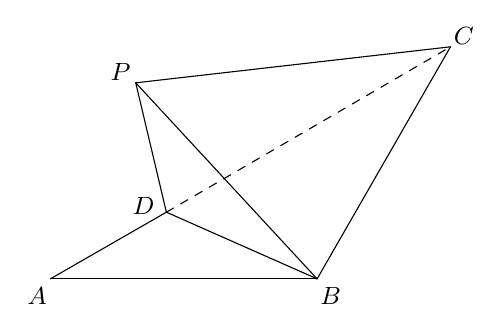
\begin{tikzpicture}[line cap=round,line join=round,font=\small,x=0.03515cm,y=0.03515cm]
% ===== 虚线先画（不可见棱 DC）=====
\draw[dash pattern=on 2.99pt off 2.99pt] (41.91,24.09)--(144.54,83.83);
% ===== 实线 =====
\draw (0,0)--(96.36,0);              % A-B
\draw (0,0)--(41.91,24.09);          % A-D
\draw (96.36,0)--(41.91,24.09);      % B-D
\draw (41.91,24.09)--(30.84,70.82);  % D-P
\draw (30.84,70.82)--(144.54,83.83); % P-C
\draw (30.84,70.82)--(96.36,0);      % P-B
\draw (96.36,0)--(144.54,83.83);     % B-C
% ===== 标注（照源字形框中心，显式坐标）=====
\node[anchor=center,inner sep=0] at (-4.73,-6.06) {\(A\)};
\node[anchor=center,inner sep=0] at (101.26,-6.06) {\(B\)};
\node[anchor=center,inner sep=0] at (149.35,87.67) {\(C\)};
\node[anchor=center,inner sep=0] at (33.70,26.40) {\(D\)};
\node[anchor=center,inner sep=0] at (25.38,74.66) {\(P\)};
\end{tikzpicture}
\end{center}
\nopagebreak[4]
\Needspace{4\baselineskip}
\textbf{解析}

建系使平面 \(ABC\) 为 \(z=0\)：取 \(B=(0,0,0)\)，\(A=(2,0,0)\)；由 \(\angle ABC=120^{\circ}\)、\(BC=2\) 得 \(C=(-1,\sqrt{3},0)\)。设 \(D=A+t(C-A)=\left(2-3t,\sqrt{3}t,0\right)\)（\(t\in[0,1]\)），则 \(DA=2\sqrt{3}\,t\)。

\Needspace{5\baselineskip}
平面 \(BCD\) 即平面 \(ABC\)，\([\triangle BCD]=(1-t)[\triangle ABC]=\sqrt{3}(1-t)\)。由 \(PB=2\)、\(PD=DA\)，点 \(P\) 在两球面的交圆上；该交圆所在平面垂直于 \(BD\)、故竖直，\(P\) 到平面 \(ABC\) 的最大距离即交圆半径

\nopagebreak[4]
\[
h_{\max}=\dfrac{\sqrt{3}\,t}{\sqrt{1-3t+3t^{2}}}.
\]

\Needspace{5\baselineskip}
于是

\nopagebreak[4]
\[
V(t)=\dfrac{1}{3}\sqrt{3}(1-t)\cdot\dfrac{\sqrt{3}\,t}{\sqrt{1-3t+3t^{2}}}=\dfrac{t(1-t)}{\sqrt{1-3t+3t^{2}}}.
\]

\Needspace{5\baselineskip}
令 \(V'(t)=0\)，得 \(6t^{3}-9t^{2}+7t-2=0\)，即 \((2t-1)(3t^{2}-3t+2)=0\)；二次因子判别式 \(9-24<0\)，故唯一驻点 \(t=\dfrac{1}{2}\)。端点处 \(V(0)=V(1)=0\)，故最大值

\nopagebreak[4]
\[
V_{\max}=V\left(\dfrac{1}{2}\right)=\dfrac{1/4}{\sqrt{1/4}}=\dfrac{1}{2}.
\]

\gkanswer{答案：\(\dfrac{1}{2}\)}

\end{answer}
\begin{answer}
\gksolhead{15}{}

\textbf{题目}：

已知向量 \(\mathbf{a}\)，\(\mathbf{b}\)，\(|\mathbf{a}|=1\)，\(|\mathbf{b}|=2\)，若对任意单位向量 \(\mathbf{e}\)，均有 \(|\mathbf{a}\cdot\mathbf{e}|+|\mathbf{b}\cdot\mathbf{e}|\leqslant\sqrt{6}\)，则 \(\mathbf{a}\cdot\mathbf{b}\) 的最大值是 \(\underline{\qquad}\)。

\Needspace{4\baselineskip}
\textbf{解析}

\Needspace{5\baselineskip}
设 \(|\boldsymbol{a}|=1\)，\(|\boldsymbol{b}|=2\)，夹角 \(\theta\)，则 \(\boldsymbol{a}\cdot\boldsymbol{b}=2\cos\theta\)。取 \(\boldsymbol{e}=(\cos\varphi,\sin\varphi)\)（可先证 \(\boldsymbol{e}\) 在 \(\boldsymbol{a}\)，\(\boldsymbol{b}\) 张成的平面内取到最大），则

\nopagebreak[4]
\[
|\boldsymbol{a}\cdot\boldsymbol{e}|+|\boldsymbol{b}\cdot\boldsymbol{e}|=|\cos\varphi|+2|\cos(\varphi-\theta)|.
\]

\Needspace{5\baselineskip}
分片求最大值得 \(M(\theta)=\sqrt{5+4\cos\theta}\)。条件 \(M(\theta)\leqslant\sqrt{6}\) 即 \(5+4\cos\theta\leqslant 6\)，故 \(\cos\theta\leqslant\dfrac{1}{4}\)。于是

\nopagebreak[4]
\[
\boldsymbol{a}\cdot\boldsymbol{b}=2\cos\theta\leqslant\dfrac{1}{2},
\]

且 \(\cos\theta=\dfrac{1}{4}\) 时等号可取，故最大值是 \(\dfrac{1}{2}\)。

\gkanswer{答案：\(\dfrac{1}{2}\)}

\end{answer}
\begin{answer}
\gksolhead{16}{}

\textbf{题目}：

在 \(\triangle ABC\) 中，内角 \(A\)，\(B\)，\(C\) 所对的边分别为 \(a\)，\(b\)，\(c\)。已知 \(b+c=2a\cos B\)。

（1） 证明：\(A=2B\)；

（2） 若 \(\triangle ABC\) 的面积 \(S=\dfrac{a^{2}}{4}\)，求角 \(A\) 的大小。

\Needspace{4\baselineskip}
\textbf{解析}

\gksubpart{(1)}

\Needspace{5\baselineskip}
由正弦定理，\(b+c=2a\cos B\) 化为 \(\sin B+\sin C=2\sin A\cos B\)。左端和差化积：

\nopagebreak[4]
\[
\sin B+\sin C=2\sin\dfrac{B+C}{2}\cos\dfrac{B-C}{2}=2\cos\dfrac{A}{2}\cos\dfrac{B-C}{2},
\]

\Needspace{5\baselineskip}
右端 \(=4\sin\dfrac{A}{2}\cos\dfrac{A}{2}\cos B\)。约去 \(\cos\dfrac{A}{2}>0\)，并用 \(C=\pi-A-B\) 化 \(\cos\dfrac{B-C}{2}=\sin\left(B+\dfrac{A}{2}\right)\)，得

\nopagebreak[4]
\[
\sin\left(B+\dfrac{A}{2}\right)=2\sin\dfrac{A}{2}\cos B\Longrightarrow\sin B\cos\dfrac{A}{2}=\sin\dfrac{A}{2}\cos B\Longrightarrow\sin\left(B-\dfrac{A}{2}\right)=0.
\]

因 \(0<B<\pi\)，\(-\dfrac{\pi}{2}<B-\dfrac{A}{2}<\pi\)，故 \(B-\dfrac{A}{2}=0\)，即 \(A=2B\)。

\gksubpart{(2)}

\Needspace{5\baselineskip}
由 \(S=\dfrac{1}{2}bc\sin A=\dfrac{a^{2}}{4}\)，取 \(a=k\sin 2B\)，\(b=k\sin B\)，\(c=k\sin 3B\)（\(C=\pi-3B\)，\(0<B<\dfrac{\pi}{3}\)），得

\nopagebreak[4]
\[
\dfrac{1}{2}k^{2}\sin B\sin 3B\sin 2B=\dfrac{1}{4}k^{2}\sin^{2}2B\Longrightarrow 2\sin B\sin 3B=\sin 2B\Longrightarrow\sin 3B=\cos B.
\]

解 \(\sin 3B=\sin\left(\dfrac{\pi}{2}-B\right)\)，在 \(B\in\left(0,\dfrac{\pi}{3}\right)\) 内得 \(B=\dfrac{\pi}{8}\) 或 \(B=\dfrac{\pi}{4}\)，故 \(A=2B=\dfrac{\pi}{4}\) 或 \(\dfrac{\pi}{2}\)（两解均满足题设）。

\gkanswer{答案（1）：见解析版}

\gkanswer{答案（2）：\(A=\dfrac{\pi}{4}\) 或 \(\dfrac{\pi}{2}\)（两解均满足题设）。}

\end{answer}
\begin{answer}
\gksolhead{17}{}

\textbf{题目}：

如图，在三棱台 \(ABC-DEF\) 中，平面 \(BCFE\perp\) 平面 \(ABC\)，\(\angle ACB=90^{\circ}\)，\(BE=EF=FC=1\)，\(BC=2\)，\(AC=3\)。

（1） 求证：\(BF\perp\) 平面 \(ACFD\)；

（2） 求二面角 \(B-AD-F\) 的平面角的余弦值。
\nopagebreak[4]
\begin{center}% 第 17 题三棱台图：按固定源 PDF 矢量路径换算（1 pt → 0.03515 cm）。
% 原点取顶点 A（源页 (980.7578, 532.9297) pt），y 向上。
% 顶点：A(0,0)、B(109.37,−41.43)、C(152.25,0)、D(65.52,37.58)、E(118.04,21.68)、F(143.57,37.58)。
% 实线 8 段（含题图额外画出的 BF——题干要求证 BF⊥平面 ACFD）；虚线 1 段：AC（被遮挡的底棱）。无箭头。
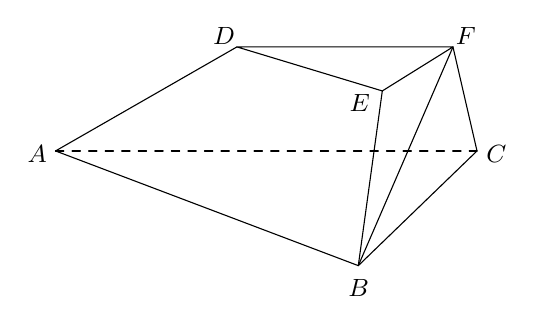
\begin{tikzpicture}[line cap=round,line join=round,font=\small,x=0.03515cm,y=0.03515cm]
% ===== 虚线先画（底棱 AC）=====
\draw[dash pattern=on 2.99pt off 2.99pt] (0,0)--(152.25,0);
% ===== 实线 =====
\draw (109.37,-41.43)--(0,0);        % BA
\draw (109.37,-41.43)--(152.25,0);   % BC
\draw (65.52,37.58)--(0,0);          % DA
\draw (118.04,21.68)--(109.37,-41.43); % EB
\draw (143.57,37.58)--(152.25,0);    % FC
\draw (109.37,-41.43)--(143.57,37.58); % BF（题图额外线段）
\draw (118.04,21.68)--(143.57,37.58)--(65.52,37.58)--cycle; % 上底 DEF（EF、FD、DE）
% ===== 标注（照源字形框中心，显式坐标）=====
\node[anchor=center,inner sep=0] at (-6.60,-1.06) {\(A\)};
\node[anchor=center,inner sep=0] at (109.52,-49.49) {\(B\)};
\node[anchor=center,inner sep=0] at (159.27,-1.06) {\(C\)};
\node[anchor=center,inner sep=0] at (60.84,41.46) {\(D\)};
\node[anchor=center,inner sep=0] at (109.87,17.20) {\(E\)};
\node[anchor=center,inner sep=0] at (148.20,41.46) {\(F\)};
\end{tikzpicture}
\end{center}
\nopagebreak[4]
\Needspace{4\baselineskip}
\textbf{解析}

\gksubpart{(1)}

由 \(\angle ACB=90^{\circ}\) 得 \(AC\perp BC\)；又平面 \(BCFE\perp\) 平面 \(ABC\)，交线为 \(BC\)，故 \(AC\perp\) 平面 \(BCFE\)，特别地 \(AC\perp BF\)。

\Needspace{5\baselineskip}
建系：\(B=(0,0,0)\)，\(C=(2,0,0)\)，\(A=(2,3,0)\)，平面 \(BCFE\) 取为 \(y=0\)；由 \(BE=EF=FC=1\)、\(EF\parallel BC\)、\(BC=2\) 得 \(E=\left(\dfrac{1}{2},0,\dfrac{\sqrt{3}}{2}\right)\)，\(F=\left(\dfrac{3}{2},0,\dfrac{\sqrt{3}}{2}\right)\)。于是

\nopagebreak[4]
\[
\overrightarrow{BF}=\left(\dfrac{3}{2},0,\dfrac{\sqrt{3}}{2}\right),\qquad\overrightarrow{CF}=\left(-\dfrac{1}{2},0,\dfrac{\sqrt{3}}{2}\right),\qquad\overrightarrow{BF}\cdot\overrightarrow{CF}=0,
\]

即 \(BF\perp CF\)。\(AC\) 与 \(CF\) 是平面 \(ACFD\) 内相交于 \(C\) 的两条直线，故 \(BF\perp\) 平面 \(ACFD\)。

\gksubpart{(2)}

三棱台由棱锥被平行于底面的截面截得，相似比为 \(\dfrac{|EF|}{|BC|}=\dfrac{1}{2}\)，故 \(D=E+\dfrac{1}{2}(A-B)=\left(\dfrac{3}{2},\dfrac{3}{2},\dfrac{\sqrt{3}}{2}\right)\)。

\Needspace{5\baselineskip}
取平面角：令 \(\boldsymbol{u}=\dfrac{\overrightarrow{AD}}{|\overrightarrow{AD}|}=\dfrac{(-1,-3,\sqrt{3})}{\sqrt{13}}\)，把 \(\overrightarrow{AB}\)、\(\overrightarrow{AF}\) 沿 \(\boldsymbol{u}\) 方向分解，得垂直于棱 \(AD\) 的两个向量

\nopagebreak[4]
\[
\boldsymbol{v}_{B}=\overrightarrow{AB}-(\overrightarrow{AB}\cdot\boldsymbol{u})\boldsymbol{u}=\dfrac{1}{13}\left(-15,-6,-11\sqrt{3}\right),
\]

\nopagebreak[4]
\[
\boldsymbol{v}_{F}=\overrightarrow{AF}-(\overrightarrow{AF}\cdot\boldsymbol{u})\boldsymbol{u}=\dfrac{1}{26}\left(9,-12,-9\sqrt{3}\right).
\]

\Needspace{5\baselineskip}
则二面角 \(B-AD-F\) 的平面角的余弦

\nopagebreak[4]
\[
\cos\langle\boldsymbol{v}_{B},\boldsymbol{v}_{F}\rangle=\dfrac{\boldsymbol{v}_{B}\cdot\boldsymbol{v}_{F}}{|\boldsymbol{v}_{B}||\boldsymbol{v}_{F}|}=\dfrac{\sqrt{3}}{4}.
\]

（法向量法复核：平面 \(ABD\) 与平面 \(ADF\) 的法向量 \(n_{1}=\left(\dfrac{3\sqrt{3}}{2},-\sqrt{3},-\dfrac{3}{2}\right)\)、\(n_{2}=\left(\dfrac{3\sqrt{3}}{4},0,\dfrac{3}{4}\right)\) 给出同值 \(\dfrac{\sqrt{3}}{4}\)。）

\gkanswer{答案（1）：见解析版}

\gkanswer{答案（2）：二面角 \(B-AD-F\) 的平面角的余弦值为 \(\dfrac{\sqrt{3}}{4}\)。}

\end{answer}
\begin{answer}
\gksolhead{18}{}

\textbf{题目}：

\Needspace{5\baselineskip}
已知 \(a\geqslant 3\)，函数 \(F(x)=\min\{2|x-1|,\ x^{2}-2ax+4a-2\}\)，其中

\nopagebreak[4]
\[
\min\{p,q\}=\begin{cases}
p, & p\leqslant q, \\
q, & p>q.
\end{cases}
\]

（1） 求使得等式 \(F(x)=x^{2}-2ax+4a-2\) 成立的 \(x\) 的取值范围；

（2） ① 求 \(F(x)\) 的最小值 \(m(a)\)；

　　② 求 \(F(x)\) 在区间 \([0,6]\) 上的最大值 \(M(a)\)。

\Needspace{4\baselineskip}
\textbf{解析}

记 \(g(x)=2|x-1|\)，\(h(x)=x^{2}-2ax+4a-2\)，则 \(F(x)=\min\{g(x),h(x)\}\)。

\gksubpart{(1)}

\(F(x)=h(x)\iff h(x)\leqslant g(x)\)。

当 \(x\geqslant 1\) 时化为 \(x^{2}-(2a+2)x+4a\leqslant 0\)，即 \((x-2)(x-2a)\leqslant 0\)，故 \(x\in[2,2a]\)（\(a\geqslant 3\) 时 \(2a\geqslant 6\)）；当 \(x<1\) 时相应二次不等式解区间的左端点大于 \(1\)，与 \(x<1\) 无交。故所求范围为 \([2,2a]\)。

\gksubpart{(2)}

\Needspace{5\baselineskip}
\textbf{①} 由 \(F(1)=\min\{0,2a-3\}=0\)（\(a\geqslant 3\)）与 \(F(a)=\min\{2a-2,h(a)\}=h(a)=-a^{2}+4a-2\)（\(a\geqslant 2\) 时 \(h(a)\leqslant 2a-2\)），得

\nopagebreak[4]
\[
m(a)=\min\{0,4a-a^{2}-2\}=\begin{cases}
0, & 3\leqslant a\leqslant 2+\sqrt{2}, \\
4a-a^{2}-2, & a>2+\sqrt{2}.
\end{cases}
\]

\Needspace{5\baselineskip}
\textbf{②} 由 (1)，在 \([2,6]\) 上 \(F=h\)；在 \([0,2]\) 上 \(F\leqslant g\leqslant 2\) 且 \(F(0)=2\)。故

\nopagebreak[4]
\[
M(a)=\max\left\{2,\ \max_{x\in[2,6]}h(x)\right\}=\max\{2,\ h(2),\ h(6)\}=\max\{2,\ 34-8a\},
\]

\Needspace{5\baselineskip}
即

\nopagebreak[4]
\[
M(a)=\begin{cases}
34-8a, & 3\leqslant a\leqslant 4, \\
2, & a>4.
\end{cases}
\]

\gkanswer{答案（1）：\(x\in[2,2a]\)（当 \(x\geqslant 1\) 时化为 \((x-2)(x-2a)\leqslant 0\)；当 \(x<1\) 时无解）。}

\gkanswer{答案（2）：① 当 \(3\leqslant a\leqslant 2+\sqrt{2}\) 时 \(m(a)=0\)，当 \(a>2+\sqrt{2}\) 时 \(m(a)=4a-a^{2}-2\)（因 \(F(1)=0\) 恒成立，最小值取 \(\min\{0,\,4a-a^{2}-2\}\)）；② 当 \(3\leqslant a\leqslant 4\) 时 \(M(a)=34-8a\)，当 \(a>4\) 时 \(M(a)=2\)。}

\end{answer}
\begin{answer}
\gksolhead{19}{}

\textbf{题目}：

如图，设椭圆 \(\dfrac{x^{2}}{a^{2}}+y^{2}=1\)（\(a>1\)）。

（1） 求直线 \(y=kx+1\) 被椭圆截得的线段长（用 \(a\)，\(k\) 表示）；

（2） 若任意以点 \(A(0,1)\) 为圆心的圆与椭圆至多有 3 个公共点，求椭圆离心率的取值范围。
\nopagebreak[4]
\begin{center}% 第 19 题椭圆坐标图：按固定源 PDF 矢量路径换算（1 pt → 0.03515 cm）。
% 原点取椭圆中心 O（源页 (692.9102, 202.0039) pt，即两轴交点），y 向上。
% 椭圆半轴 56.6719/34.0020（轴比 ≈5:3，源为示意画法），线宽 0.8pt（源为其余图元 2 倍）；
% x 轴左 −76.51 右至箭头 76.51、y 轴下 −56.67 上至箭头 59.51（均穿出椭圆，左右不对称照源）；
% 标签 y/A/x/O 四处；A 标于椭圆上顶点（对应题设 A(0,1)）。无实心点、无刻度。
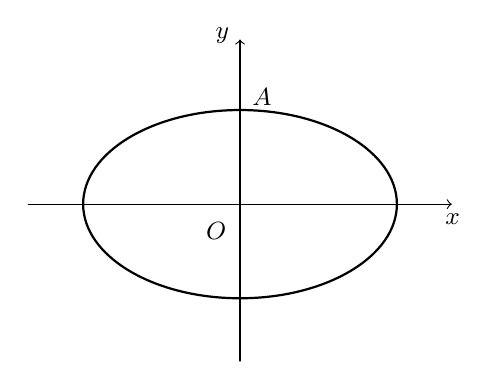
\begin{tikzpicture}[line cap=round,line join=round,font=\small,x=0.03515cm,y=0.03515cm]
% 坐标轴
\draw[->] (-76.51,0)--(76.51,0);
\draw[->] (0,-56.67)--(0,59.51);
% 椭圆（线宽 0.8，与源一致）
\draw[line width=0.8pt] (0,0) ellipse (56.67 and 34.00);
% ===== 标注（照源字形框中心，显式坐标）=====
\node[anchor=center,inner sep=0] at (-6.39,60.94) {\(y\)};
\node[anchor=center,inner sep=0] at (7.91,38.75) {\(A\)};
\node[anchor=center,inner sep=0] at (76.80,-5.57) {\(x\)};
\node[anchor=center,inner sep=0] at (-8.59,-9.66) {\(O\)};
\end{tikzpicture}
\end{center}
\nopagebreak[4]
\Needspace{4\baselineskip}
\textbf{解析}

\gksubpart{(1)}

\Needspace{5\baselineskip}
直线 \(y=kx+1\) 过椭圆上顶点 \(A(0,1)\)。代入椭圆方程：

\nopagebreak[4]
\[
\dfrac{x^{2}}{a^{2}}+(kx+1)^{2}=1\Longrightarrow x\left[\left(\dfrac{1}{a^{2}}+k^{2}\right)x+2k\right]=0,
\]

\Needspace{5\baselineskip}
另一交点横坐标 \(x_{0}=-\dfrac{2ka^{2}}{1+a^{2}k^{2}}\)，故截得线段长

\nopagebreak[4]
\[
|AP|=|x_{0}|\sqrt{1+k^{2}}=\dfrac{2a^{2}|k|\sqrt{1+k^{2}}}{1+a^{2}k^{2}}.
\]

\gksubpart{(2)}

椭圆上纵坐标为 \(y\) 的点到 \(A(0,1)\) 的距离平方为 \(\psi(y)=a^{2}(1-y^{2})+(y-1)^{2}\)。以 \(A\) 为圆心的圆与椭圆至少 4 个公共点，等价于存在两个不同的 \(y\in(-1,1)\) 使 \(\psi\) 取同值；故「任意圆至多 3 个公共点」等价于 \(\psi(y)\) 在 \((-1,1)\) 上单射。

\Needspace{5\baselineskip}
\(\psi(y)=(1-a^{2})y^{2}-2y+(a^{2}+1)\) 开口向下（\(a>1\)），顶点 \(y_{0}=-\dfrac{1}{a^{2}-1}<0\) 在 \((-1,1)\) 上单射当且仅当 \(y_{0}\leqslant-1\)，即 \(a^{2}\leqslant 2\)。故 \(1<a\leqslant\sqrt{2}\)，离心率

\nopagebreak[4]
\[
e=\dfrac{\sqrt{a^{2}-1}}{a}\in\left(0,\dfrac{\sqrt{2}}{2}\right].
\]

\gkanswer{答案（1）：截得的线段长为 \(\dfrac{2a^{2}|k|\sqrt{1+k^{2}}}{1+a^{2}k^{2}}\)。}

\gkanswer{答案（2）：离心率的取值范围是 \(\left(0,\dfrac{\sqrt{2}}{2}\right]\)。}

\end{answer}
\begin{answer}
\gksolhead{20}{}

\textbf{题目}：

设数列 \(\{a_{n}\}\) 满足 \(\left|a_{n}-\dfrac{a_{n+1}}{2}\right|\leqslant 1\)，\(n\in\mathbf{N}^{*}\)。

（1） 证明：\(|a_{n}|\geqslant 2^{n-1}(|a_{1}|-2)\)，\(n\in\mathbf{N}^{*}\)；

（2） 若 \(|a_{n}|\leqslant\left(\dfrac{3}{2}\right)^{n}\)，\(n\in\mathbf{N}^{*}\)，证明：\(|a_{n}|\leqslant 2\)，\(n\in\mathbf{N}^{*}\)。

\Needspace{4\baselineskip}
\textbf{解析}

记 \(a_{n+1}=2a_{n}-2\varepsilon_{n}\)，其中 \(|\varepsilon_{n}|\leqslant 1\)。

\gksubpart{(1)}

\Needspace{5\baselineskip}
递推展开：\(a_{n}=2^{n-1}a_{1}-\sum\limits_{k=1}^{n-1}2^{\,n-k}\varepsilon_{k}\)。由三角不等式，

\nopagebreak[4]
\[
|a_{n}|\geqslant 2^{n-1}|a_{1}|-\sum\limits_{k=1}^{n-1}2^{\,n-k}\geqslant 2^{n-1}|a_{1}|-(2^{n}-2)=2^{\,n-1}\left(|a_{1}|-2\right)+2\geqslant 2^{\,n-1}\left(|a_{1}|-2\right).
\]

\gksubpart{(2)}

\Needspace{5\baselineskip}
反设存在 \(m\) 使 \(|a_{m}|>2\)。由反向三角不等式 \(|a_{n+1}|\geqslant 2|a_{n}|-2\) 得 \(|a_{n+1}|-2\geqslant 2\left(|a_{n}|-2\right)\)，故 \(|a_{n}|>2\)（\(n\geqslant m\)）且

\nopagebreak[4]
\[
|a_{n}|\geqslant 2+2^{\,n-m}\left(|a_{m}|-2\right)>2^{\,n-m}\left(|a_{m}|-2\right).
\]

\Needspace{5\baselineskip}
与 \(|a_{n}|\leqslant\left(\dfrac{3}{2}\right)^{n}\) 联立得 \(2^{\,n-m}\left(|a_{m}|-2\right)<\left(\dfrac{3}{2}\right)^{n}\)，即

\nopagebreak[4]
\[
|a_{m}|-2<2^{m}\left(\dfrac{3}{4}\right)^{n}.
\]

右端随 \(n\to\infty\) 趋于 \(0\)，故 \(|a_{m}|-2\leqslant 0\)，与 \(|a_{m}|>2\) 矛盾，从而对一切 \(n\in\mathbf{N}^{*}\)，\(|a_{n}|\leqslant 2\)。

\gkanswer{答案（1）：见解析版}

\gkanswer{答案（2）：见解析版}

\end{answer}